\documentclass[a4paper,12pt, english]{article}
\usepackage[T1]{fontenc}
\usepackage[utf8]{inputenc}
\usepackage{graphicx}
\usepackage{babel}
\usepackage{amsmath}
\usepackage{ulem}
\usepackage{a4wide}

\usepackage{listings}
\usepackage{tabularx}
\usepackage{tabulary}

\usepackage{caption}
\usepackage{subcaption}

\begin{document}

\begin{titlepage}
\begin{center}
\textsc{\Large Computational Physics, Project 5}\\[0.5cm]
\textsc{Candidate number}\\[0.5cm]

\end{center}
\end{titlepage}

\begin{abstract}
Results and conclusion
http://young.physics.ucsc.edu/115/leapfrog.pdf
\end{abstract}

\section*{$N$-body simulation of an open galactic cluster}

\subsection*{Introduction}

Throughout this project we will develop a code to perform simulations of an open cluster using Newtonian gravity. We will consider the evolution by following the motion of its constituent stars. This interacting classical system require integrating Newton's equation of motion over a long period of time starting from some initial conditions. This type of simulations are called "N-body" simulations. 

First we will compare the stability of two different methods for solving differential equations; the fourth order Runge-Kutta and the Leap-Frog method. When we are looking at a system with a large number of particles we are more interested in the statistical properties than the individual motion of each of the particles. This means that the stability of the solution method is more important than its short term accuracy.

First we implement the Newtonian two-body problem in three-dimensions. We choose to look at a hypothetical solar system, with only one planet, the Earth, orbiting the Sun. We will check the stability of the two numerical methods for different time steps and time scales. 

Thereafter we will adapt our code to simulate a simple model of how an open cluster is made from the gravitational collapse and interaction among a large number of stars. In this simulation we will assume what is called a "cold collapse", that is that the particles starts with little or no initial velocity. We will rewrite the code so that it works for an arbitrary number of particles. We will start with a uniform (random) distribution within a sphere of a given radius $R_0$. The masses of the particles will be randomly distributed by a Gaussian distribution around ten solar masses with a standard deviation of one solar mass. From our simulations we will extract information about the systems energies. We will look at energy conservation and the ejected particles and their associated energies for a different number of particles $N$. 
To take care of the numerical instability that arises when the particles come very close, we will insert a smoothing function.      


\subsection*{Theory}

The only force in this problem is gravity, given by Newton's law of gravitation. The force between two objects with masses $M_1$ and $M_2$ is 

\[
F = \frac{GM_1 M_2}/{r^2}
\]

where $r$ is the distance between them and $G$ the gravitational constant. 

In one dimension Newton's second law yields this second-order differential equation

$$m\frac{d^2x}{dt^2} = F(x,t)$$

We can rewrite the second-order ordinary differential equation as a set of coupled first order differential equations. 
We know that the velocity and the acceleration is connected to the position by the time derivative so that

\[
\frac{dx}{dt} = v(x,t) \hspace{1cm}\mathrm{and}\hspace{1cm}
\frac{dv_x}{dt} = \frac{F(x,t)}{M} = a(x,t)
\]

Performing a Taylor expansion we get 
\[
x(t+h) = x(t) + hx^{(1)} + \frac{h^2}{2}x^{(2)}(t) + O(h^3)
\]

To calculate the next time step of the system we will use two methods for numerically integrating differential equations; the Runga-Kutta method and the Leap-Frog method.

We implement these methods for a Newtonian two-body system, looking at the Earth's orbit around the Sun. In our simulation we assume that the Sun and the Earth is the only objects in the system, and choose the initial conditions such that the orbit of the Earth should be circular.

For circular motion we know that the force must obey the following relation 
$$\frac{M_{Earth}v^2}{r} = F_G = \frac{GM_{sun}M_{Earth}}{r^2}$$ where $v$ is the velocity of the Earth. 
For circular orbit the velocity of the Earth is $v = \frac{2 \pi r}{1 year}$, where the distance between Sun and Earth is $r = 1 AU$. Hence $v = 2 \pi (AU/years)$. Rearranging the equation we find
$$v^2r = GM_{sun} = 4 \pi ^2 AU^3/years^2$$

We know that for circular motion the velocity will be tangential. It follows that if we choose the initial conditions $ x = 1 AU $ and $ y = 0$, with velocities $v_x = 0$ and $v_y = v_{tangential} = 2 \pi AU/year$ we will get circular orbit.    

The next task in the project was to build a model of an open cluster. An open cluster is a group up to a few thousand gravitationally bound stars created from the collapse of a molecular cloud. In our model we work with a few hundred particles. We start the particles with no initial velocity, that is we simulate a so-called "cold collapse". Since the objects have no relative motion with respect to each other initially, the cluster collapses by its gravity. 

Since the distribution of the clumps in the cluster is spherical and uniform, all the clumps will collapse simultaneously.
In a system like this the evolution of the system leads to a singularity after a finite time as $N -> \inf$, since all the mass arrives at the origin after a time $\tau_{crunch}$. The time of the collapse is given by $$\tau_{crunch} = \sqrt{\frac{3 \pi}{32G \rho_0}},$$ where $\rho_0$ is the initial mass density. 

Our numerical simulation has a finite number of particles $N$, and thus the singularity does not occur. Even if we had the ability to make the simulation for an infinite number of particles, we have approximated the objects as point particles. In the limit where $N -> \inf$, and keeping $\rho$ constant, we should get a continuous fluid. However, looking at the particles as point particles, we will not get the uniformly distributed "lump" of mass which leads to the system collapse into a singularity.     

Using $\tau_{crunch}$ as an unit of time, we can find $G$ in these units. 

\[
\tau_{crunch} = \sqrt{\frac{3 \pi}{32 G \rho_0}} = 1
\]

which gives 

\[
\frac{3 \pi}{32G \rho_0} = 1 \hspace{1mm} \Rightarrow \hspace{1mm} G = \frac{3 \pi}{32 \rho_0}
\]

We have that 
\[
\rho_0 = \frac{\Sigma M}{V} = \frac{\mu N}{ \frac{4}{3} \pi R_0^3} 
\]

where we have used that the total mass is the average mass of the particles, $/mu$, times the number of particle, $N$. 

We thus have
\[
G = \frac{3 \pi}{32} \frac{4 \pi R_0^3}{3 \mu N} = \frac{\pi^2 R_0^ 3}{8 \mu N}
\]


When two of the particles come very close we will find that a time step that is reasonable for larger distances now is far too large for our calculations. This because we will get very large accelerations when the particles have close encounters, and thus the necessity for very small time steps. To take care of this numerical instability we introduce a smoothing function. We modify the Newtonian force to make it finite at short ranges
\[
F_{mod} = - \frac{GM_1M_2}{r^2 + \epsilon^2}
\]

The parameter $\epsilon$ is a small real constant which we set to be $\epsilon = 0.15 ly$. We see that setting $\epsilon = 0$ will give us back the standard Newtonian equation of motion. We can justify the correction to the pure Newtonian force by noting that our particles do not represent actual point particles but rather mass distribution of some finite extent. 

With this modified force the code does not integrate accurately trajectories in which particles have close encounters, but on a macroscopic scale this trajectories does not play any significant role.   


With this modification in place we will look at the particles that are bound. The particles that are ejected will have larger kinetic than potential energy, and thus our bound particles are the ones with a total energy less than zero. For these particles we will find the distribution of potential and kinetic energy. We will check if our results are in agreement with the virial theorem that states that for a bound gravitational system in equilibrium we have 
\[
2\langle K\rangle = -\langle V \rangle
\]

To find the potential energy for one particle, we sum over the gravitational force working on it from all the other particles. If we take the sum over the potential energy of all the particles, we get the contribution from the gravitational force twice. Thus the potential energy contribution to the total energy is half of the sum over the potential energy for each particle.
To find the total energy of the system we thus sum over the kinetic energy and half the potential energy of all the particles. In addition we have to subtract the potential energy of the ejected particles, so all effect from these particles is disregarded in our equilibrium system.

We also wish to plot the radial density of the particles in the equilibrium state. To extract the information needed from our simulations, we first find the mass and position of all bound particles. From this we can calculate the center of mass, summing over the mass and position of each particle and dividing by the total mass. 


$$	x_{cm} = \frac{1}{M_{tot}} \Sigma M_i x_i $$
$$	y_{cm} = \frac{1}{M_{tot}} \Sigma M_i y_i $$
$$	z_{cm} = \frac{1}{M_{tot}} \Sigma M_i z_i $$

We find the radius of the bound particles relative to the center of mass
\[
r_i = \sqrt{(x_i - x_{cm})^2 + (y_i - y_{cm})^2 + (z_i - z_{cm})^2 }
\]

We then have a sphere centred around the center of mass with particles placed in different distances around it. To find the radial density we can divide the sphere into difference shells. The density of each shell will then be the number of particles within this shell, that is particles in a distance $r_{i-1}$ to $r_i$, divided by the volume of the shell. The volume of each shell will be given by the volume of a sphere with the outer radius subtracted by the volume of a sphere with the inner radius.

\[ 
d(r_{shell}) = \frac{q}{ \frac{4}{3} \pi r_i^3 - \frac{4}{3} \pi r_{i-1}^3}  
 \]
 
where $q$ is the number of particles within the shell. 

\begin{figure}
	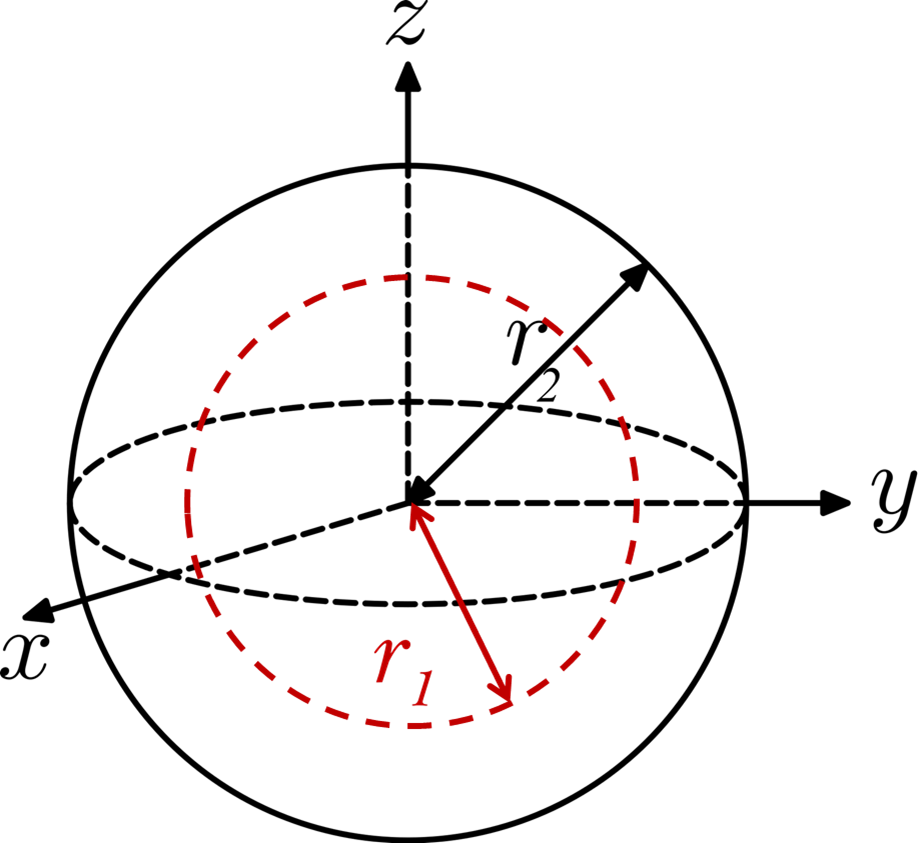
\includegraphics[scale=0.5]{sphere.png}
	\caption{\textit{Illustration from $ http://en.wikipedia.org/wiki/List_of_moments_of_inertia$}
	\label{fig:sphere}
\end{figure}
	

The radial distribution of particles in this kind of collapse can often be fit very well with the simple expression
\[ 
n(r) = \frac{n_0}{\left(1 +\left(\frac{r}{r_0}\right)^4\right)}.
\]

 
\subsection*{Method}

Both the Runge-Kutta and the Leap-Frog solver are methods that advances the solution from $x(t)$ to $x(t+h) = x(t) + hv(t)$ where $h$ is the step length to the new point we are calculating. The step is defined by splitting an interval of size $N$ in to sub-intervals $h = \frac{b-a}{N}$. With this step and the derivative of $x$ we can construct the next value of the function. 

If we were only to use the derivative at the beginning of each interval when calculating the next step, as in Euler's method, the error in each calculation will be in the power $O(\Delta t^2)$. The Runge-Kutta method improves the approximation by using trial steps within each interval to make a better estimate of the derivative. The fourth-order Runge-Kutta method requires four evaluations in each interval $\Delta t$, and thus reduces the error to the power $O(\Delta t^5$.  

 
\subsubsection*{The Runge-Kutta method}

The Runge-Kutta solver is a method for solving ordinary differential equations for which we know the initial values. In this project the motion of the planets are described by a second-order differential equation of the position as a function of time. We want to find the propagation of this function forward in time starting from the given initial values. 

Taylor series expansion of a function $x$ around $t$ gives
$$ x(t+ \Delta t) = x(t) + \frac{dx}{dt} \Delta t + \frac{1}{2} + \frac{d^2 x}{d^2 t} (\Delta t)^2 + \cdots $$

If we assume a reasonable smooth function $x(t)$ and a small interval $\Delta t$ we can approximate $x(t)$ to $x(t + \Delta t)$ as long as we know the derivatives of $x(t)$. 

In a general Runge-Kutta method we approximate the slope by different function evaluations with different weights.

When using the Runge-Kutta four approximation one estimates the slopes at four points, once at the initial point, twice at the trial midpoint and once at the trial endpoint. 
$$ k_1 = \Delta t f(t_i,x_i) \\
k_2 = \Delta t f(t_i + \Delta t /2, x_i + k_1/2) \\
k_3 = \Delta t f(t_i + \Delta t/2, x_i + k_2/2) \\
k_4 = \Delta t f(t_i + \Delta t, x_i + k3) $$

These four derivatives constitute the next value in our propagation
$$x_{i+1} = x_i + \frac{1}{6} (k_1 + 2(k_2+k_3) + k_4$$ 
  
\begin{figure}[h!]
  \centering    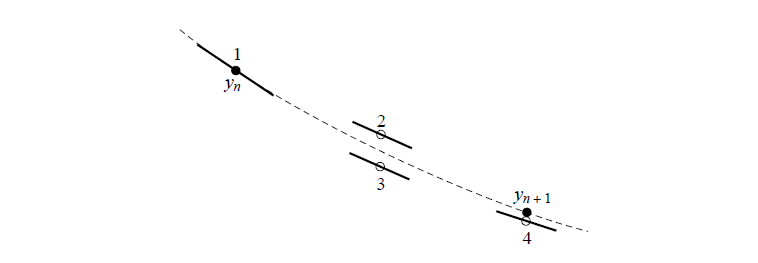
\includegraphics[scale=0.5]{rk4.png}
  \caption{\textit{Fourth-order Runge-Kutta method. In each step the derivative is evaluated four times:
once at the initial point, twice at trial midpoints, and once at a trial endpoint. From these derivatives the
final function value is calculated. }}
\end{figure}


 \begin{lstlisting}[title={Function RK4}]
void Solver:: RungeKutta4() {

    vec k1, k2, k3, k4;
    vec C = zeros(values*n);
 
    for(int i=0; i<N; i++) {

        Solver::SolveSystem(A);	 // Calculates the time derivatives 											of A 
        k1 = dAdt;				
        C = A + k1*(dt/2);		 // Updates A in a "temporary" 
        								vector C
        Solver::SolveSystem(C);
       
        k2 = dAdt;
        C = A + k2*(dt/2);

        Solver::SolveSystem(C);
        k3 = dAdt;
        C = A + k3*dt;

        Solver::SolveSystem(C);
        k4 = dAdt;

        A += (dt/6.)*(k1 + 2*(k2+k3) + k4);
      
        }
    }
}
\end{lstlisting} 

\subsubsection*{The Leap-Frog method}

The Leap-Frog scheme uses another approach to reach the best approximation. In the first step you use the initial conditions to calculate the velocity at the middle of the interval.
$$ v(t + h/2) = v(t) + \frac{h}{2} a(t). $$
Then you use this value to calculate the new position 
$$x(t+h) = x(t) + hv(t + h/2).$$
Finally you calculate the velocity at the end of the interval 
$$v(t+h) = v(t+h/2) + \frac{h}{2} a(t+h).$$   

 \begin{lstlisting}[title={Function Leap Frog}]
void Solver::LeapFrog() {

    double x, y, z, vx, vy, vz, ax, ay, az, ax_new, ay_new, az_new;

    vec vx_new(n);
    vec vy_new(n);
    vec vz_new(n);

    for(int j=0; j<N; j++) {

        Solver::SolveSystem(A);

        for(int i=0; i<n; i++) {

            int vi = values*i;

            x = A(vi);
            y = A(vi+1);
            z = A(vi+2);

            vx = dAdt(vi);
            vy = dAdt(vi+1);
            vz = dAdt(vi+2);

            ax = dAdt(vi+3);                        // ax(t)
            ay = dAdt(vi+4);                        // ay(t)
            az = dAdt(vi+5);                        // az(t)

            vx_new(i) =  vx + (dt/2)*ax;            // vx(t+dt/2)
            vy_new(i) =  vy + (dt/2)*ay;            // vy(t+dt/2)
            vz_new(i) =  vz + (dt/2)*az;            // vz(t+dt/2)

            A(vi)   = x + dt*vx_new(i);             // x(t+dt)
            A(vi+1) = y + dt*vy_new(i);             // y(t+dt)
            A(vi+2) = z + dt*vz_new(i);             // z(t+dt)
        }

        Solver::SolveSystem(A);

        for(int i=0; i<n; i++) {

            int vi = values*i;

            ax_new = dAdt(vi+3);                   // ax(t+dt)
            ay_new = dAdt(vi+4);                   // ay(t+dt)
            az_new = dAdt(vi+5);                   // az(t+dt)

            A(vi+3) = vx_new(i) + (dt/2)*ax_new;    // vx(t+h)
            A(vi+4) = vy_new(i) + (dt/2)*ay_new;    // vy(t+h)
            A(vi+5) = vz_new(i) + (dt/2)*az_new;    // vz(t+h)
        }
    }
}
\end{lstlisting}

\subsection*{Implementing the methods}
In my program I have two external classes; one that holds the values of various constants, like the gravitational constant, the masses of the different objects and so on, and one class "Planet". The latter creates an instance when called upon that contains information of the initial position and velocity and the mass corresponding to the object. For instance, 

\begin{lstlisting}[title={Making of instance}]
planet Earth = planet(1.0, 0.0, 0.0, 0.0, 2.*pi, 0.0, M_earth);
\end{lstlisting} 

makes an instance Earth that contains the initial $x, y, z$ - positions and $v_x, v_y, v_z$ - velocities and the mass of the Earth.

I then create a vector $A$ that contains the initial positions, $(x,y,z)$, and the velocities, $(v_x,v_y,v_z)$, for all objects.

\[ A = \left( \begin{array}{c}
x - object \hspace*{0.5mm} 1\\
y - object \hspace*{0.5mm} 1\\
z - object \hspace*{0.5mm} 1 \\
vx - object \hspace*{0.5mm} 1\\
vy -object \hspace*{0.5mm}  1\\
vz - object \hspace*{0.5mm} 1 \\
x - object \hspace*{0.5mm} 2\\
... \\
vz - object \hspace*{0.5mm} n \end{array} \right)\]    

I have a function that finds the time derivative of these values, $dAdt$. The time derivative of the position is simply the velocity, and that value is already saved in $A$ and easy to obtain. To find the acceleration, that is the time derivative of the velocities, I use Newtons second law. For each planet we then sum over the gravitational forces working on it from all the other objects, and thus find the acceleration. 

To calculate the time propagation of the objects, I use the Runge-Kutta and the Leap-Frog methods discussed above. Both calculating the propagation forward in time starting from the given initial conditions. 

My program is built in such a way that the function calculating the derivatives, the Runge-Kutta and the Leap-Frog solver works for different lengths of the vector $A$. Thus to change my program from the two-body system to the $N$-body system it is only the initial value of $A$ that needs changing.

For the two-body system the initial conditions is quite straight forward

 \begin{lstlisting}[title={Initial conditions two-body system}]
 vec A = zeros(values*n);
 vec dAdt = zeros(values*n);
 vec M = zeros(n);

 planet Earth = planet(1.0, 0.0, 0.0, 0.0, 2.*pi, 0.0, M_earth);
 planet Sun = planet(0.0, 0.0, 0.0, 0.0, 0.0, 0.0, M_sun);
 planet B[n];

 B[0] = Earth;
 B[1] = Sun;

  // initial conditions

  for (int i=0; i<n; i++) {
        int j = values*i;		// values = 2*dimensionality
       
        A(j)   = B[i].x0;                     // x - position
        A(j+1) = B[i].y0;                     // y - position
        A(j+2) = B[i].z0;                     // z - position
        A(j+3) = B[i].vx;                     // vx - velocity
        A(j+4) = B[i].vy;                     // vy - velocity
        A(j+5) = B[i].vz;                     // vz - velocity

        M(i)   = B[i].M;
        
    }
 
 \end{lstlisting}
 
 
For the $N$-body system, however, the initial conditions are a bit more challenging. We wish to place our $N$ particles in a uniform, random distribution within a sphere of radius $R_0$. The initial velocities are easy. We will simulate what is called a "cold collapse", and start our particles with no initial velocity. The particles should be randomly distributed by a Gaussian distribution around ten solar masses with a standard deviation of one solar mass.  


\subsubsection*{Uniformly distributed random coordinates within a sphere and randomly distributed mass}

To find the coordinates of the particles we used the function $ran2$ that was available from the web page. It yields a random number between 0 and 1 when called upon with a negative seed. For our purpose we wish to convert these numbers into coordinates of uniformly distributed particles within a sphere of radius $R_0$. 

To do this one can use spherical coordinates
\begin{align}
x = r sin \theta cos \phi \\
y = r sin \theta sin \phi \\
z = r cos \theta
\end{align}

where $ \theta \hspace{0.5mm} \epsilon \hspace{0.5mm} [0, \pi], \phi \hspace{0.5mm} \epsilon \hspace{0.5mm} [0, 2\pi], r \hspace{0.5mm} \epsilon \hspace{0.5mm} [0, R_0]$. 
 
We then use the fact that the volume element should be the same for any coordinate system. We introduce three new variables with a uniform distribution between 0 and 1, and write the volume element in terms of these coordinates. We get
\[
r^2 sin \theta dr d \theta d \phi = Adudvdw
\]

where $A$ is just a constant and $u, v, w \hspace{0.5mm} \epsilon \hspace{0.5mm} [0,1]$. When separating the variables we get three equations   

\[
r^2dr = adu \hspace{1cm}\mathrm{,}\hspace{1cm}
sin \theta = bdv \hspace{1cm}\mathrm{,}\hspace{1cm}
d \phi = cdw
\]

Integrating up we find that
\[
\phi = 2 \pi w  \hspace{1cm}\mathrm{and}\hspace{1cm}
r = R_0 \sqrt[3]{u}  \hspace{1cm}\mathrm{and}\hspace{1cm}
   \theta = arccos(1-2v) 
\]

After calculating these values it is easy to transform back to $(x,y,z)$-coordinates using the expressions for the spherical coordinates.


The mass of the objects should be randomly distributed by a Gaussian distribution around ten solar masses with a standard deviation of a solar mass. We used the function $gaussian_deviate$, which has a standard deviation $ \sigma = 1$ and is centred around zero. To get our wanted distribution with a standard deviation of $1$ and centration around ten solar masses we used  
$$ M = \sigma gaussian_deviate() + \mu $$
where $\sigma = 1$ and $\mu = 10$. 

\begin{lstlisting}[title={Initial conditions for the N-body system}]
    for (int i=0; i<N; i++) {

        u = ran2(&idum);
        v = ran2(&idum);
        w = ran2(&idum);

        phi = 2*pi*w;
        r = R0*cbrt(u);
        theta = acos(1-2*v);

        x = r*sin(theta)*cos(phi);
        y = r*sin(theta)*sin(phi);
        z = r*cos(theta);

        int j = values*i;

        A(j)   = x;                     // x - position
        A(j+1) = y;                     // y - position
        A(j+2) = z;                     // z - position
        A(j+3) = 0.0;                     // vx - velocity
        A(j+4) = 0.0;                     // vy - velocity
        A(j+5) = 0.0;                     // vz - velocity

        M(i) = sigma*gaussian_deviate(&idum) + mu;
    }
  
\end{lstlisting}


\subsection*{Radial density}
To calculate the radial density we look at the total energy for each object at a time t. Looping over the energies we pick put the objects that has a negative total energy and thus are bound. Using the mass and position of these particles we then calculate the center of mass. We then write the radius relative to the center of mass to a file.   


   
\subsection*{Results}

Running our program for the two methods we see that with the right choice of time step both yields the wanted trajectory with the Earth in circular orbit around the Sun. See figure \ref{dt_0.002}. 

\begin{figure}
        \centering
        \begin{subfigure}[b]{0.6\textwidth}
                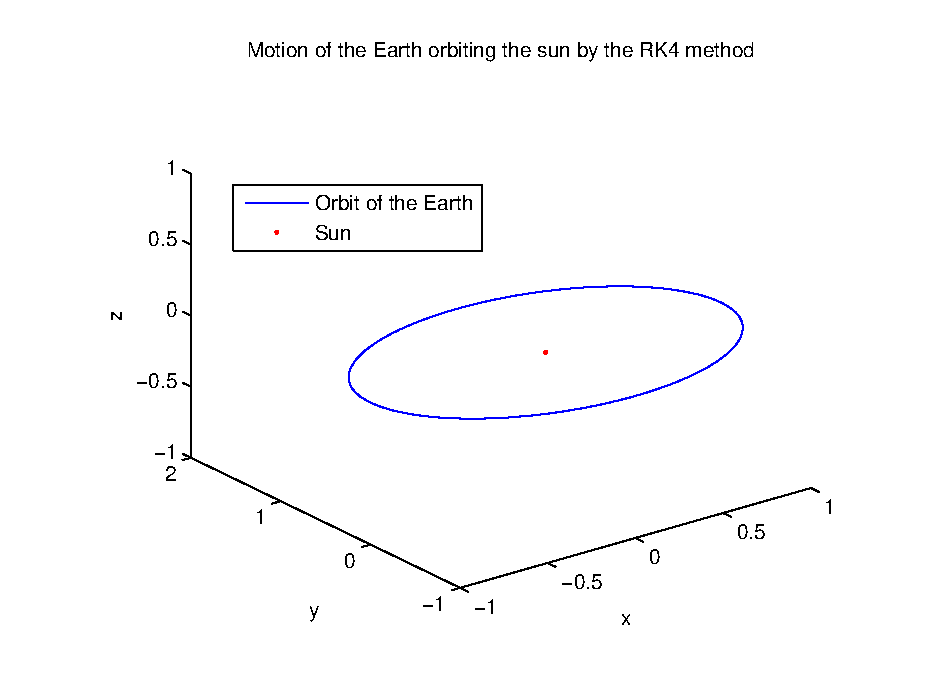
\includegraphics[width=\textwidth]{RK4_n_1000_t_2.pdf}
                \caption{Runge-Kutta method}
                \label{fig:RK4_dt_0.002}
        \end{subfigure}%
 )
        \begin{subfigure}[b]{0.6\textwidth}
                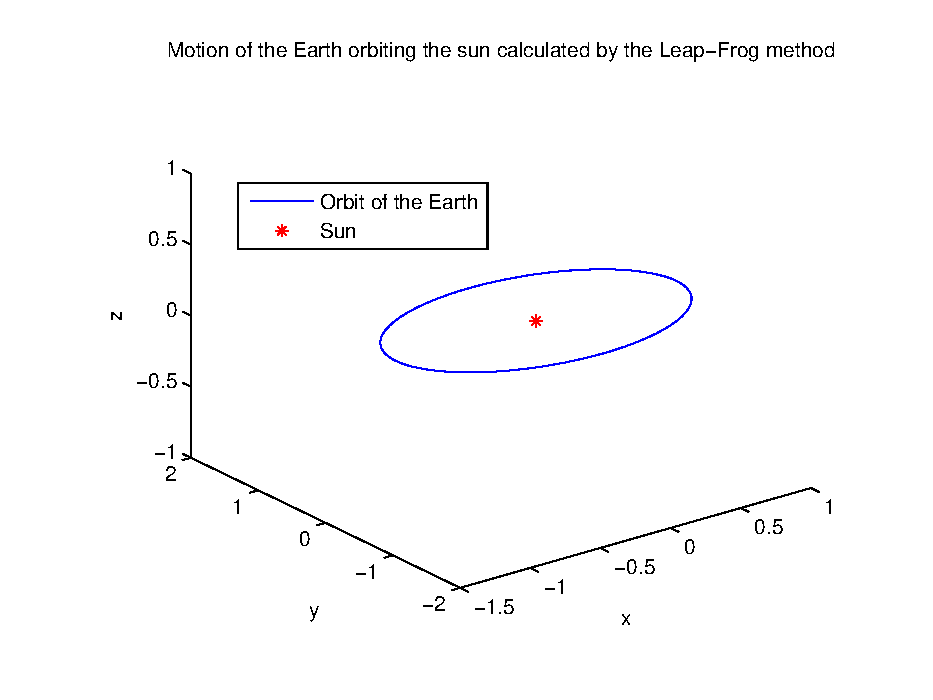
\includegraphics[width=\textwidth]{LF_n_1000_t_2.pdf}
                \caption{Leap-Frog method}
                \label{fig:LF_dt_0.002}
        \end{subfigure}
        \caption{Motion of the Earth orbiting the Sun calculated for two years with a time step $\Delta t = 0.002$}
\label{dt_0.002}
\end{figure}

However, when running for different time steps we found that our algorithm highly depends on the choice of step. The program will not yield the wanted result if we do not choose the right time step. From the figures \ref{dt_0.002} we see that time step $\Delta t = 0.002$ gives the wanted trajectory for both methods, while a time step of the size $\Delta t = 0.1$, \ref{dt0.1}, is unstable for both methods. 

From the figures \ref{timestep} we see that the Leap-Frog method is less vulnerable to the wrong choice of time step than the Runge-Kutta solver. The radius should be constant at $1 AU$, but for large time steps we see that both methods get highly unstable. We see from the figures that while the Leap-Frog method tolerates a larger time step than the Runge-Kutta method before it gets unstable. 


We see that for $\Delta t = 0.1$ the Runge-Kutta method gives a solution where the Earth starts spirals in towards the Sun. As the Earth gets too close to the Sun, a time step that was reasonable for more distant objects is far to large when we get close to the Sun. And thus we get the effect we see from figure \ref{dt0.1}; the Earth escapes from the Sun's  gravitational field. 

	
\begin{figure}
        \centering
        \begin{subfigure}[b]{0.6\textwidth}
                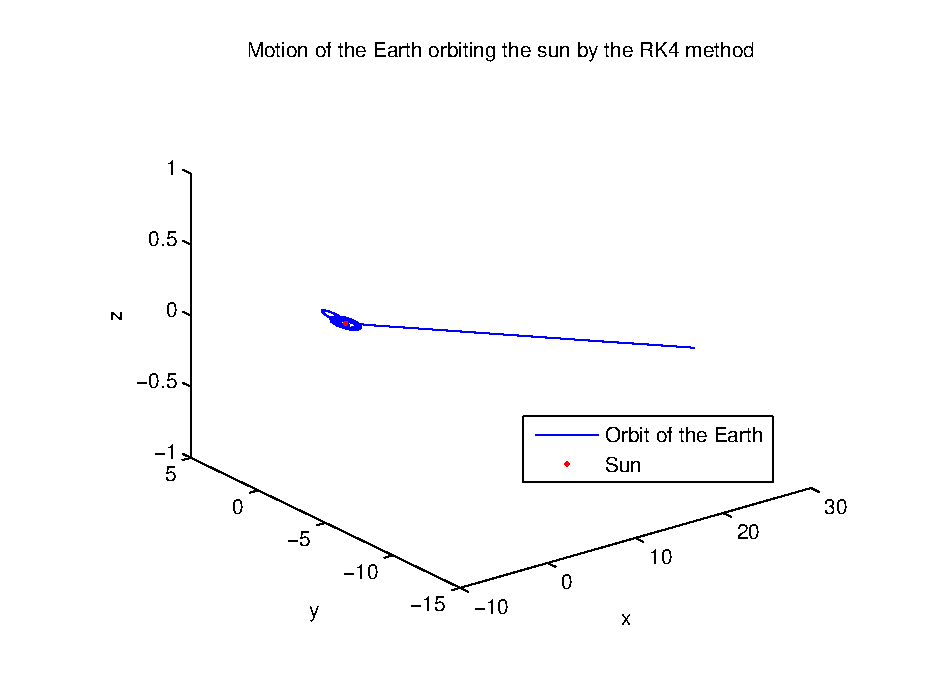
\includegraphics[width=\textwidth]{RK4_n_80_t_8.pdf}
                \caption{Runge-Kutta method}
                \label{fig:RK4_dt_0.1}
        \end{subfigure}%
        
        \begin{subfigure}[b]{0.6\textwidth}
                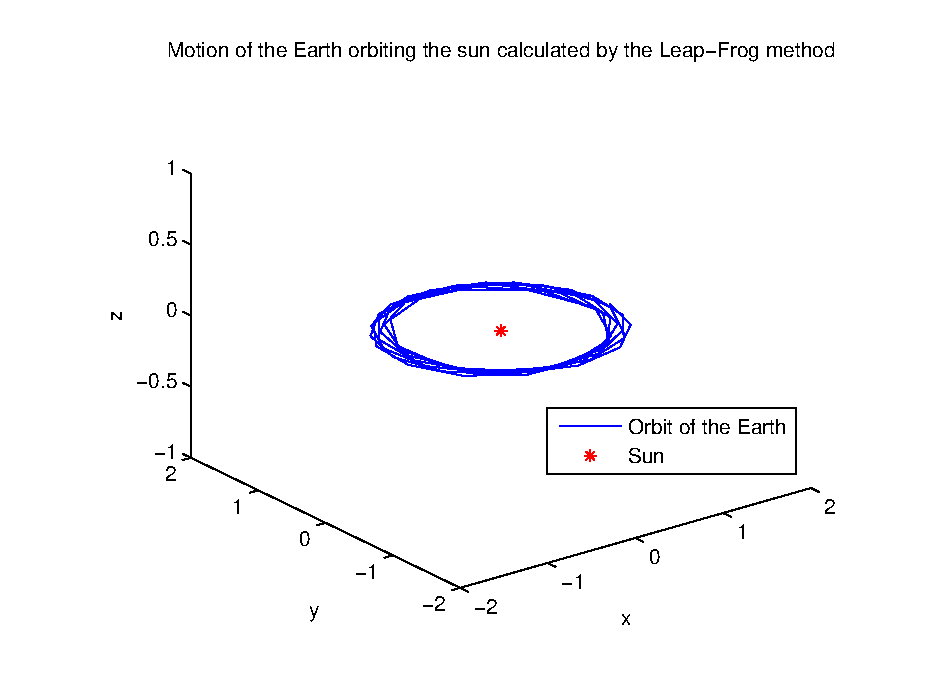
\includegraphics[width=\textwidth]{LF_n_80_t_8.pdf}
                \caption{Leap-Frog method}
                \label{fig:LF_dt_0.1}
        \end{subfigure}
        \caption{Motion of the Earth orbiting the Sun calculated for eigth years with a time step $\Delta t = 0.1$}
\label{dt0.1}   
\end{figure}

\begin{figure}
        \centering
        \begin{subfigure}[b]{0.6\textwidth}
                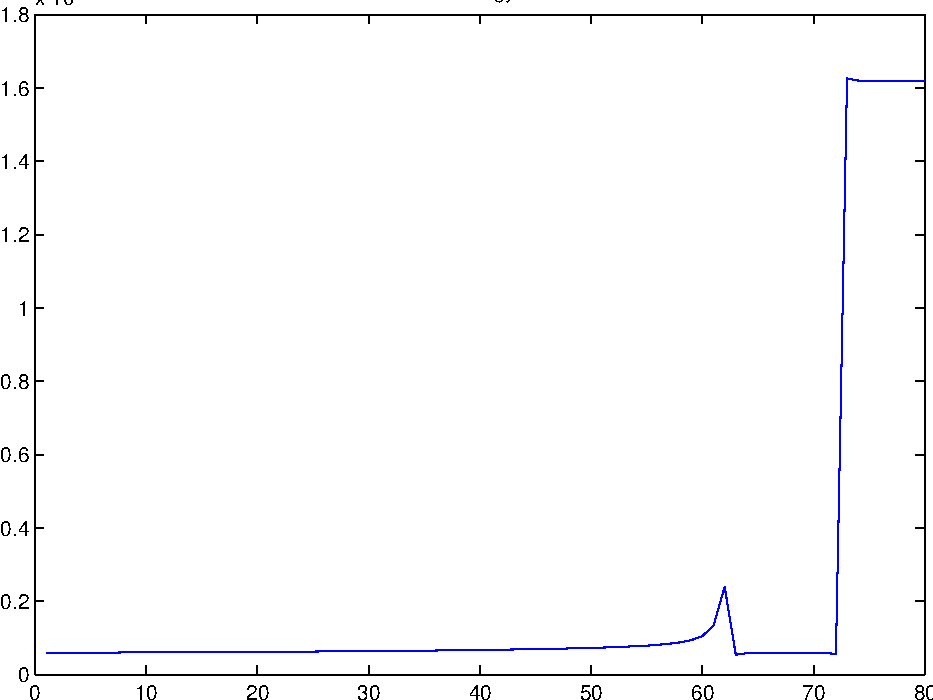
\includegraphics[width=\textwidth]{main_totE_rk4_dt_0_1.pdf}
                \caption{Runge-Kutta method absolute value of the total energy}
                \label{fig:RK4_dt_0.1}
        \end{subfigure}%
       
        \begin{subfigure}[b]{0.8\textwidth}
                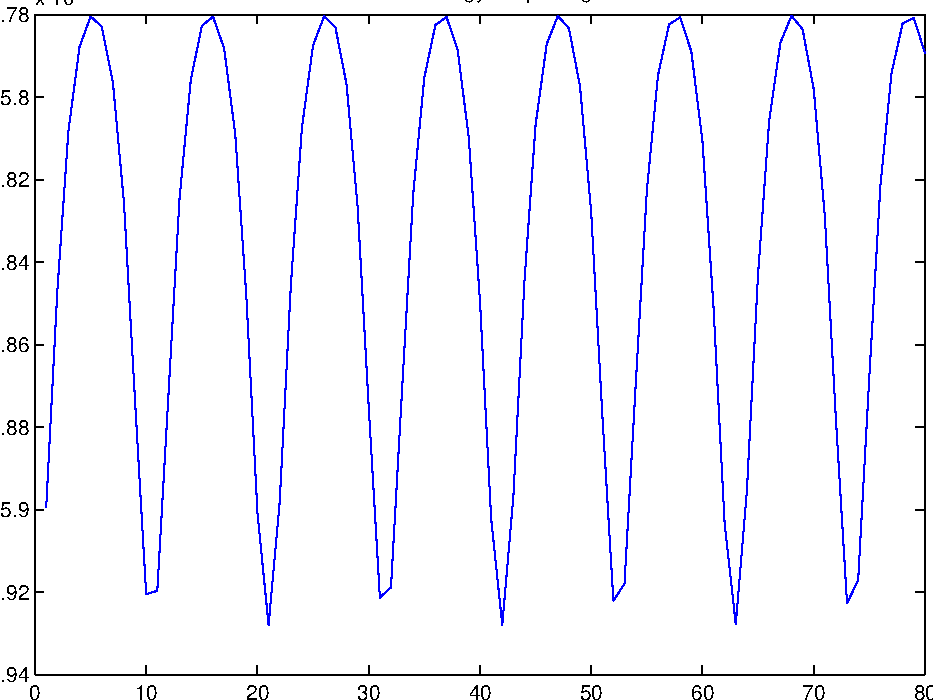
\includegraphics[width=\textwidth]{totE_main_lf_dt_0_1.pdf}
                \caption{Leap-Frog method}
                \label{fig:LF_dt_0.1}
        \end{subfigure}
        \caption{Energy for eigth years with a time step $\Delta t = 0.1$}
    
\end{figure}

	
\begin{figure}
	\begin{subfigure}
		\centering
		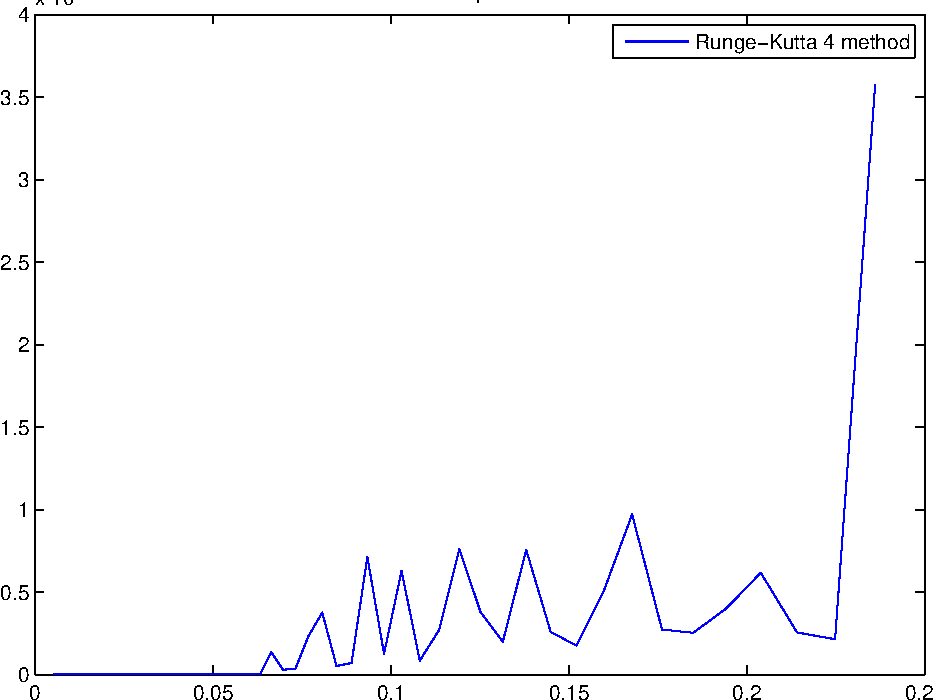
\includegraphics[scale=0.5]{timestep_rk4.pdf}
		\caption{Plot over various time steps and the maximal radius for the Runge-Kutta solver}
		\label{fig:RK4_timestep}
	\end{subfigure}

	\begin{subfigure}
		\centering
		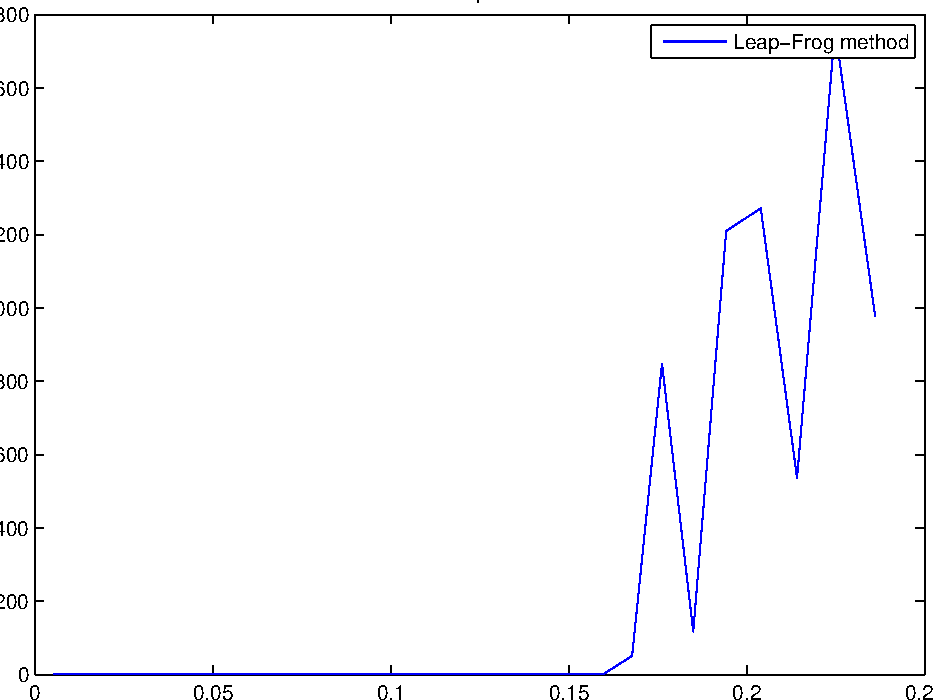
\includegraphics[scale=0.5]{timestep_LeapFrog.pdf}
		\caption{Plot over various time steps and the maximal radius for the Leap-Frog solver}
		\label{fig:LF_timestep}
	\end{subfigure}
	\label{timestep}
\end{figure}



\subsection*{ENERGY}



\begin{figure}
	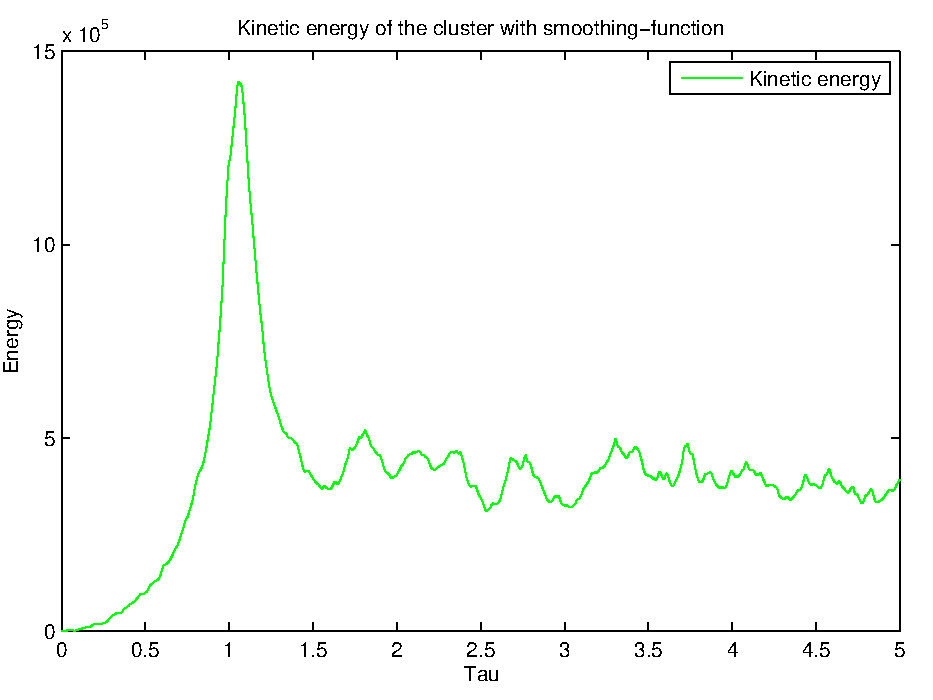
\includegraphics[scale=0.5]{kine_n1000t5.pdf}
	\caption{\textit{Total kinetic energy for the cluster with smoothing function}}
	\label{fig:sub2}
\end{figure}
\begin{figure}
	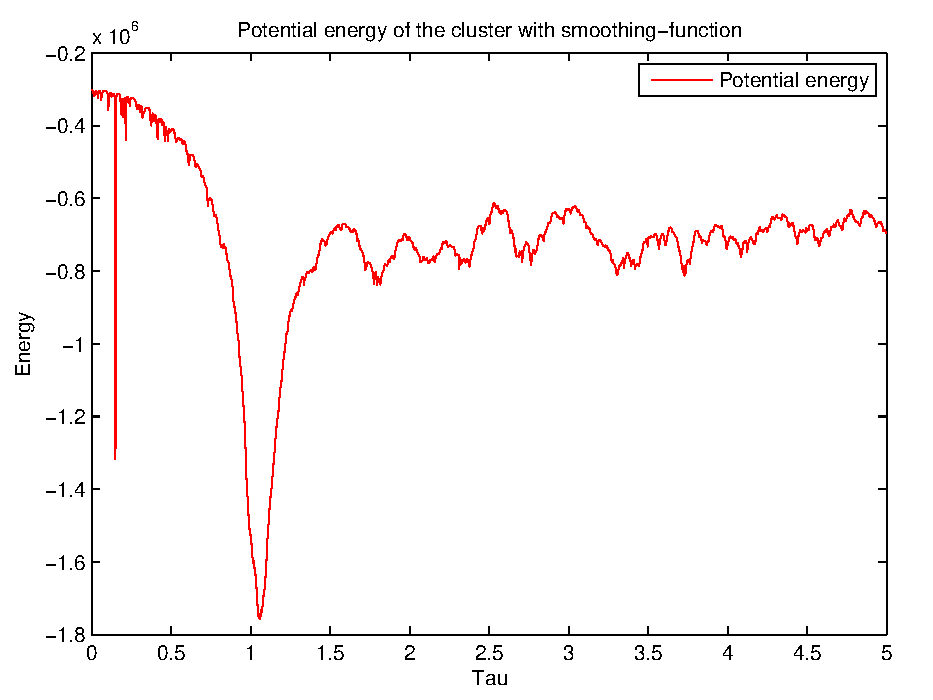
\includegraphics[scale=0.5]{pote_n1000t5.pdf}
	\caption{\textit{Total potential energy for the Cluster with smoothing function}}
	\label{fig:pote}
\end{figure}



\begin{figure}
	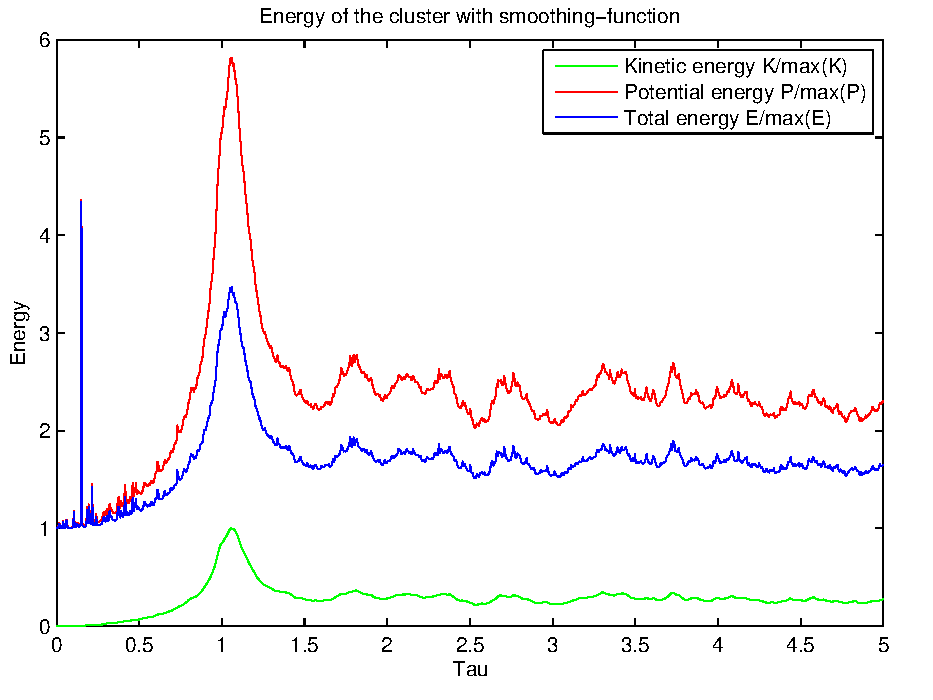
\includegraphics[scale=0.5]{energy_n1000t5_N100.pdf}
	\caption{\textit{Total kinetic energy for the cluster with smoothing function}}
	\label{fig:sub2}
\end{figure}





$$For plot av Cluster RK4 med t_f = 2 og n = 1000 --> fin animasjon av hvordan partiklene "forsvinner" når vi ikke bruker en smoothing funksjon. Samme som vi fant i prosjekt 3 når vi hadde for stort tidsteg. Partiklene kom for nære hverandre og fikk veldig stor energi --> sendt ut av gravitasjonsfeltet.   
$$





\subsection*{Conclusion}
 

http://www.ee.nthu.edu.tw/bschen/files/c16-1.pdf
\end{document}